\section{Multivariate UQ}
We now extend the univariate uncertainty quantification to multivariate solvers.  For now, we limit ourselves to the tensor product collocation space, which we acknowledge as sufficient but quite inefficient.  Improving on this approach is the significant focus for future work.  We consider uncertain vector $Y=[Y_1,Y_2,\ldots,Y_N]$ as uncertain input parameters for the solution $U(Y)$.  We expand as before, but considering $N$ uncorrelated input parameters:
\begin{equation}
U(\theta;Y)\approx U_P(\theta;Y) = \sum_{p_1=0}^{P_1}\sum_{p_2=0}^{P_2}\cdots\sum_{p_N=0}^{P_N} u_{\bar p}(\theta) \prod_{n=1}^N\psi_{p_n}(Y),
\end{equation}
where now multi-index $\bar p=[p_1,p_2,\ldots,p_N]$ denotes a single set of expansion orders, one for each variable.  The multi-index is taken from the multi-index set $\Lambda(L)$, which includes all desired multi-indices.  In the case of tensor product space,
\begin{equation}
\Lambda_\text{TP}(L)=\qty{\bar p=(p_1,\ldots,p_N):\max_{1\leq n\leq N} P_n\leq L}.
\end{equation}
This tensor product space quickly becomes unmanageably large, as the size of the index set scales as
\begin{equation}
|\Lambda_\text{TP}(L)|=(L+1)^N.
\end{equation}
However, this index set will serve to demonstrate the UQ algorithm and its capacity to treat multivariate UQ for deterministic solvers.

\subsection{Polynomial Solver: $f(x,y)$}
We once again include this case for its analytic mean and variance.  We introduce uniform uncertainty to both parameters as $x\sim\mathcal{U}(3,7),y\sim\mathcal{U}(1,6)$.  The analytic expected statistics along with the Monte Carlo and PCESC statistics are shown in Table \ref{tab: poly milt res}, and the PDFs in Fig. \ref{fig: poly milt res}
\begin{table}[H]
\begin{center}
\begin{tabular}{c c|l l}
type & runs/order & mean & variance \\ \hline
Analytic & - & $45/2$ & $81.8611111111$ \\
MC & $1\times10^7$ & 22.4962950638 & 81.8754664265 \\
SC & (1,1) & 22.5 & 81.8611111111 \\
\end{tabular}
\end{center}
\caption{Polynomial Solver, Bivariate Uniform Distribution Statistics}
\label{tab: poly milt res}
\end{table}
\begin{figure}[H]
\centering
%  \begin{subfigure}[b]{0.45 \textwidth}
   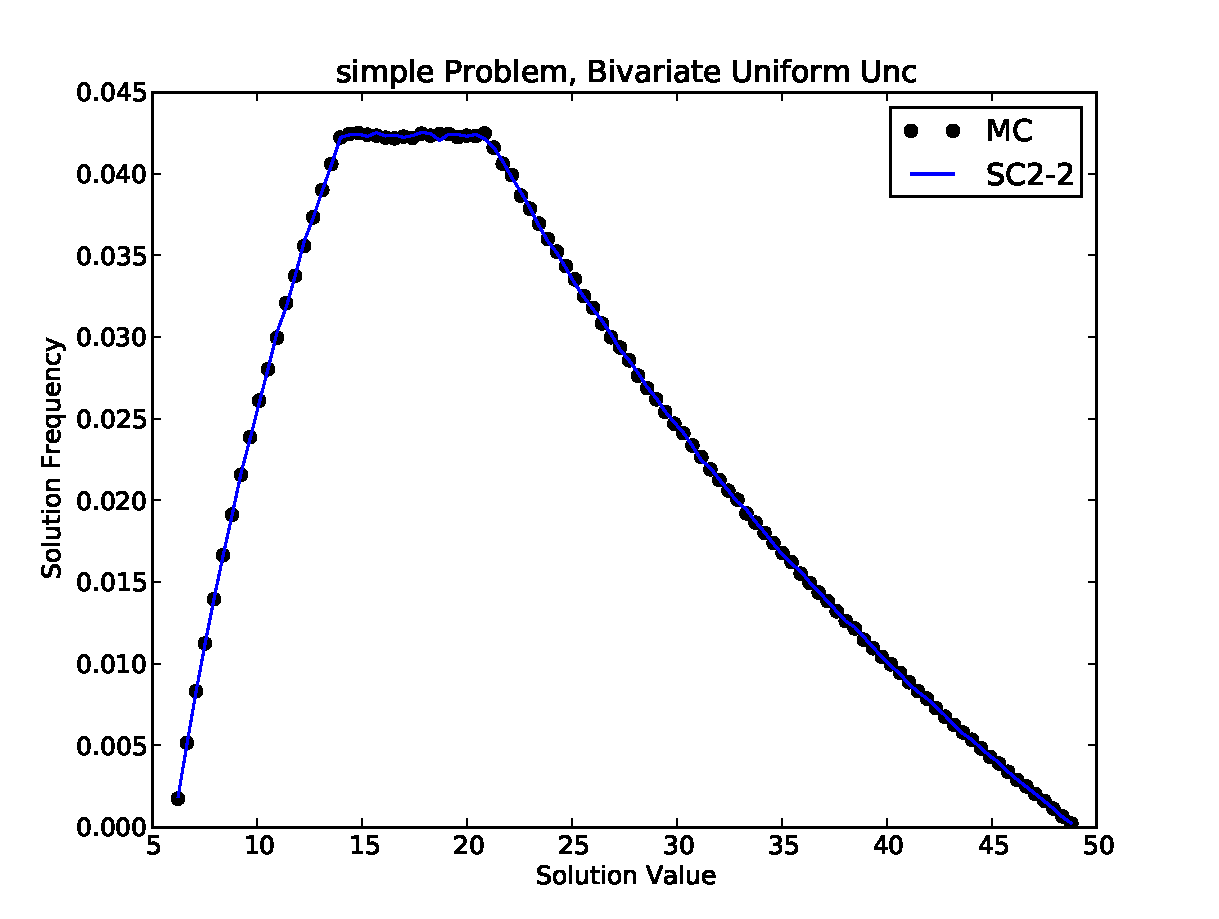
\includegraphics[width=0.5\textwidth]{../graphics/poly_2v_uniform_pdfs}
   \caption{Polynomial Solver, Bivariate Uniform PDFs}
      \label{fig: poly milt res}
%  \end{subfigure}
\end{figure}

\subsection{Source Solver: $\phi=\phi\qty(S,D,x,\Sigma_a)$}
In addition to the absorption cross section, we introduce uncertainty in the location at which the flux is measured.  This occasion might arise when the exact absorption properties of a medium are unknown and a point detector is placed with some uncertainty.  We allow the input parameters to be uncertain as $\Sigma_a\sim\mathcal{U}(0.5,1),x\sim\mathcal{U}(1.5,2.5)$.  The other two parameters remain constant as
\begin{align}
S &= 1.0 \text{ n/cm}^2\text{/s},\\
D &= 0.5 \text{ /cm}.
\end{align}
The statistical results are in Table \ref{tab: source mult res} and the PDFs in Fig. \ref{fig: source mult res}.
\begin{table}[H]
\begin{center}
\begin{tabular}{c c|l l}
type & order($\Sigma_a,x$) & mean & variance \\ \hline
MC & $1\times10^6$ & 1.24791828682 & 0.0508287413676\\
SC & (2,2) & 1.24804231569 & 0.0506451101763 \\
SC & (2,4) & 1.24804212351 & 0.0506466208388\\
SC & (4,2) & 1.24806746049 & 0.0507934845282\\
SC & (4,4) & 1.24806726831 & 0.0507949951904 \\
\end{tabular}
\end{center}
\caption{Statistics for Source Solver with Bivariate Uniform Uncertainty}
\label{tab: source mult res}
\end{table}
\begin{figure}[h]
\centering
   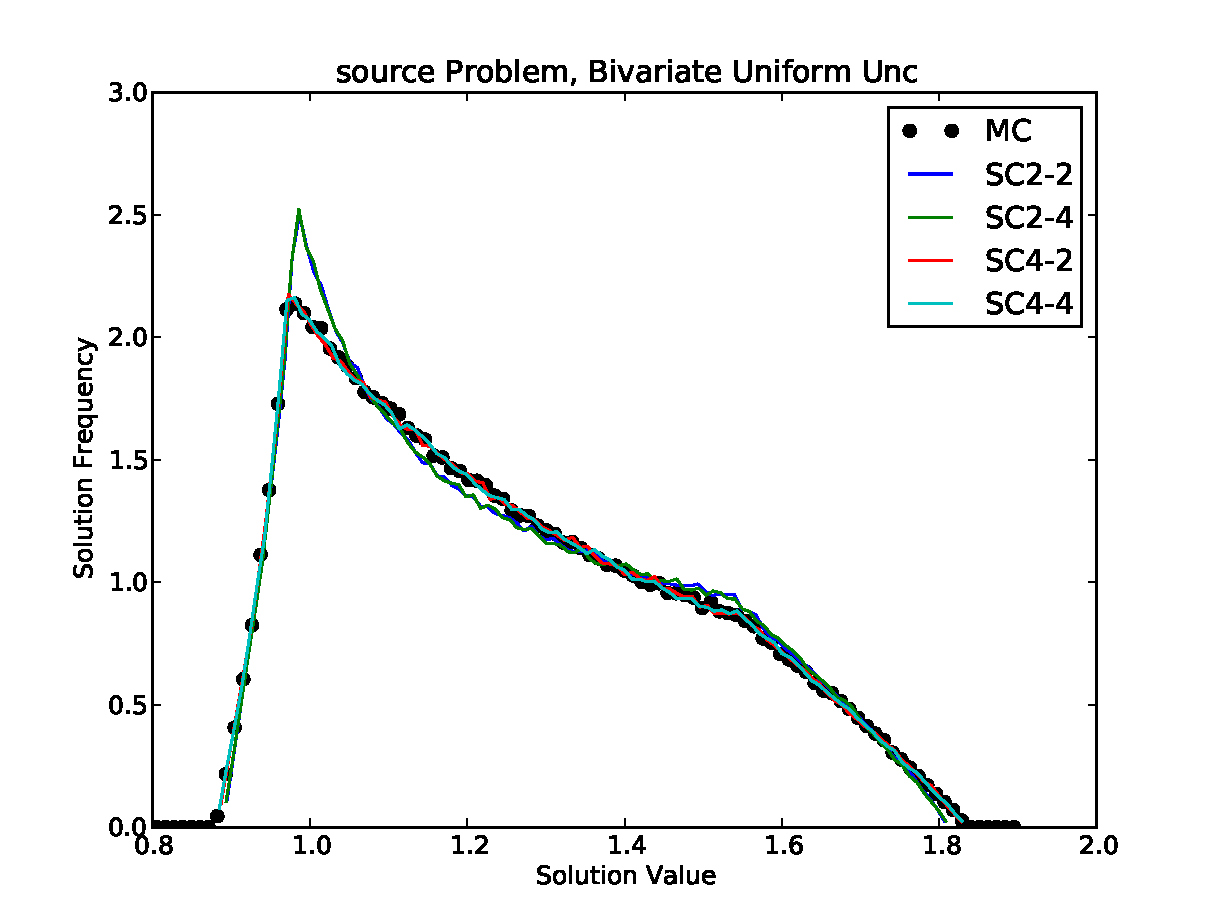
\includegraphics[width=0.5\textwidth]{../graphics/source_2v_uniform_pdfs}
\caption{Bivariate Source Solver Solution Distributions}
\label{fig: source mult res}
\end{figure}

\newpage
\subsection{Quarter Core Solver: $k=k\qty(D_g^{(R)},\xs{g,c}{R},\xs{g'\to g,s}{R},\xs{g,f}{R},\nu_g^{(R)})$}
In this case we consider five uncertain parameters simultaneously, as in Table \ref{tab:2d2g5param}.  Each was given approximately 10\% uncertainty from its mean in the benchmark problem.
\begin{table}[H]
\begin{center}
\begin{tabular}{c c c c}
Region & Energy Group & Parameter & Uncertainty \\ \hline
1 & 2 & $\Sigma_c$ & $\mathcal{U}(0.050,0.061) $\\
1 & 2 & $\Sigma_f$ & $\mathcal{U}(0.098,0.120) $\\
4 & 2 & $\Sigma_c$ & $\mathcal{U}(0.037,0.046) $\\
4 & 2 & $\Sigma_f$ & $\mathcal{U}(0.092,0.112) $\\
5 & 2 & $D$            & $\mathcal{U}(0.143,0.175) $\\
\end{tabular}
\end{center}
\caption{Quarter Core Multivariate Uncertainty Space}
\label{tab:2d2g5param}
\end{table}

We also can attempt to make informed guesses as to the appropriate expansion order of each input parameter by performing independent convergence studies for each.  Using the results from \S \ref{sec:spaceconv}, we use expansion orders based on convergence tolerance.  The results are in Table \ref{tab:2dcrit5v}.

\begin{table}[H]
\begin{center}
\begin{tabular}{c c c|l l}
type & tol & $\mathcal{P}(\Sigma_{2,c}^1,\Sigma_{2,f}^1,\Sigma_{2,c}^4,\Sigma_{2,f}^4,D^5_2)$ & mean & variance \\ \hline
MC & - & - & 0.999064586714 & 0.0262019588485 \\
SC & 1e-4 & (5, 4, 3, 3, 1) & 1.00191085676 & 0.000202816510815 \\
SC & 1e-5 & (6, 5, 4, 3, 1) & 1.00112487809 & 0.000554497293737\\
SC & 1e-6 & (8, 7, 5, 4, 2) & 1.00018130781 & 0.00245280240592 \\
SC & 1e-8 & (10, 9, 6, 4, 3) & 1.00014901416 & 0.00207327774315
\end{tabular}
\end{center}
\caption{Statistics for Multivariate Quarter Core Solver}
\label{tab:2dcrit5v}
\end{table}
The mean is converged quite swiftly.  The variance improves quickly with decreased tolerance, but there is still an order of magnitude difference between the Monte Carlo-calculated variance and the PCESC-calculated variance.  This suggests that considering only independent convergence of parameters is insufficient, and future studies will include consideration for convergence by pairwise input parameters.
